\documentclass[]{article}
\usepackage{lmodern}
\usepackage{amssymb,amsmath}
\usepackage{ifxetex,ifluatex}
\usepackage{fixltx2e} % provides \textsubscript
\ifnum 0\ifxetex 1\fi\ifluatex 1\fi=0 % if pdftex
  \usepackage[T1]{fontenc}
  \usepackage[utf8]{inputenc}
\else % if luatex or xelatex
  \ifxetex
    \usepackage{mathspec}
  \else
    \usepackage{fontspec}
  \fi
  \defaultfontfeatures{Ligatures=TeX,Scale=MatchLowercase}
\fi
% use upquote if available, for straight quotes in verbatim environments
\IfFileExists{upquote.sty}{\usepackage{upquote}}{}
% use microtype if available
\IfFileExists{microtype.sty}{%
\usepackage{microtype}
\UseMicrotypeSet[protrusion]{basicmath} % disable protrusion for tt fonts
}{}
\usepackage[margin=1in]{geometry}
\usepackage{hyperref}
\hypersetup{unicode=true,
            pdftitle={Homework 1},
            pdfauthor={Jetnisa Krasniqi, Mehdi Hirari, Rachel Louve Cerutti},
            pdfborder={0 0 0},
            breaklinks=true}
\urlstyle{same}  % don't use monospace font for urls
\usepackage{color}
\usepackage{fancyvrb}
\newcommand{\VerbBar}{|}
\newcommand{\VERB}{\Verb[commandchars=\\\{\}]}
\DefineVerbatimEnvironment{Highlighting}{Verbatim}{commandchars=\\\{\}}
% Add ',fontsize=\small' for more characters per line
\usepackage{framed}
\definecolor{shadecolor}{RGB}{248,248,248}
\newenvironment{Shaded}{\begin{snugshade}}{\end{snugshade}}
\newcommand{\KeywordTok}[1]{\textcolor[rgb]{0.13,0.29,0.53}{\textbf{#1}}}
\newcommand{\DataTypeTok}[1]{\textcolor[rgb]{0.13,0.29,0.53}{#1}}
\newcommand{\DecValTok}[1]{\textcolor[rgb]{0.00,0.00,0.81}{#1}}
\newcommand{\BaseNTok}[1]{\textcolor[rgb]{0.00,0.00,0.81}{#1}}
\newcommand{\FloatTok}[1]{\textcolor[rgb]{0.00,0.00,0.81}{#1}}
\newcommand{\ConstantTok}[1]{\textcolor[rgb]{0.00,0.00,0.00}{#1}}
\newcommand{\CharTok}[1]{\textcolor[rgb]{0.31,0.60,0.02}{#1}}
\newcommand{\SpecialCharTok}[1]{\textcolor[rgb]{0.00,0.00,0.00}{#1}}
\newcommand{\StringTok}[1]{\textcolor[rgb]{0.31,0.60,0.02}{#1}}
\newcommand{\VerbatimStringTok}[1]{\textcolor[rgb]{0.31,0.60,0.02}{#1}}
\newcommand{\SpecialStringTok}[1]{\textcolor[rgb]{0.31,0.60,0.02}{#1}}
\newcommand{\ImportTok}[1]{#1}
\newcommand{\CommentTok}[1]{\textcolor[rgb]{0.56,0.35,0.01}{\textit{#1}}}
\newcommand{\DocumentationTok}[1]{\textcolor[rgb]{0.56,0.35,0.01}{\textbf{\textit{#1}}}}
\newcommand{\AnnotationTok}[1]{\textcolor[rgb]{0.56,0.35,0.01}{\textbf{\textit{#1}}}}
\newcommand{\CommentVarTok}[1]{\textcolor[rgb]{0.56,0.35,0.01}{\textbf{\textit{#1}}}}
\newcommand{\OtherTok}[1]{\textcolor[rgb]{0.56,0.35,0.01}{#1}}
\newcommand{\FunctionTok}[1]{\textcolor[rgb]{0.00,0.00,0.00}{#1}}
\newcommand{\VariableTok}[1]{\textcolor[rgb]{0.00,0.00,0.00}{#1}}
\newcommand{\ControlFlowTok}[1]{\textcolor[rgb]{0.13,0.29,0.53}{\textbf{#1}}}
\newcommand{\OperatorTok}[1]{\textcolor[rgb]{0.81,0.36,0.00}{\textbf{#1}}}
\newcommand{\BuiltInTok}[1]{#1}
\newcommand{\ExtensionTok}[1]{#1}
\newcommand{\PreprocessorTok}[1]{\textcolor[rgb]{0.56,0.35,0.01}{\textit{#1}}}
\newcommand{\AttributeTok}[1]{\textcolor[rgb]{0.77,0.63,0.00}{#1}}
\newcommand{\RegionMarkerTok}[1]{#1}
\newcommand{\InformationTok}[1]{\textcolor[rgb]{0.56,0.35,0.01}{\textbf{\textit{#1}}}}
\newcommand{\WarningTok}[1]{\textcolor[rgb]{0.56,0.35,0.01}{\textbf{\textit{#1}}}}
\newcommand{\AlertTok}[1]{\textcolor[rgb]{0.94,0.16,0.16}{#1}}
\newcommand{\ErrorTok}[1]{\textcolor[rgb]{0.64,0.00,0.00}{\textbf{#1}}}
\newcommand{\NormalTok}[1]{#1}
\usepackage{longtable,booktabs}
\usepackage{graphicx,grffile}
\makeatletter
\def\maxwidth{\ifdim\Gin@nat@width>\linewidth\linewidth\else\Gin@nat@width\fi}
\def\maxheight{\ifdim\Gin@nat@height>\textheight\textheight\else\Gin@nat@height\fi}
\makeatother
% Scale images if necessary, so that they will not overflow the page
% margins by default, and it is still possible to overwrite the defaults
% using explicit options in \includegraphics[width, height, ...]{}
\setkeys{Gin}{width=\maxwidth,height=\maxheight,keepaspectratio}
\IfFileExists{parskip.sty}{%
\usepackage{parskip}
}{% else
\setlength{\parindent}{0pt}
\setlength{\parskip}{6pt plus 2pt minus 1pt}
}
\setlength{\emergencystretch}{3em}  % prevent overfull lines
\providecommand{\tightlist}{%
  \setlength{\itemsep}{0pt}\setlength{\parskip}{0pt}}
\setcounter{secnumdepth}{0}
% Redefines (sub)paragraphs to behave more like sections
\ifx\paragraph\undefined\else
\let\oldparagraph\paragraph
\renewcommand{\paragraph}[1]{\oldparagraph{#1}\mbox{}}
\fi
\ifx\subparagraph\undefined\else
\let\oldsubparagraph\subparagraph
\renewcommand{\subparagraph}[1]{\oldsubparagraph{#1}\mbox{}}
\fi

%%% Use protect on footnotes to avoid problems with footnotes in titles
\let\rmarkdownfootnote\footnote%
\def\footnote{\protect\rmarkdownfootnote}

%%% Change title format to be more compact
\usepackage{titling}

% Create subtitle command for use in maketitle
\newcommand{\subtitle}[1]{
  \posttitle{
    \begin{center}\large#1\end{center}
    }
}

\setlength{\droptitle}{-2em}

  \title{Homework 1}
    \pretitle{\vspace{\droptitle}\centering\huge}
  \posttitle{\par}
    \author{Jetnisa Krasniqi, Mehdi Hirari, Rachel Louve Cerutti}
    \preauthor{\centering\large\emph}
  \postauthor{\par}
      \predate{\centering\large\emph}
  \postdate{\par}
    \date{March 10, 2019}


\begin{document}
\maketitle

\subsection{Introduction}\label{introduction}

This is our first R markdown document. In this section we will do a
quick introduction about Japanese culture followed by a video and a text
to explain what we think bout it. As you will see in the third section
their will be a presentaion of what each person likes the most for
example with Jetnisa it will be japanese culture and for Mehdi will be
Arthur Conan Doyle and so on so forth. We will finish the assignement
with R syntax and references that we used for our work.

Let's take a look !

This is an introductory video aout Japan. A presentaion of common things
in japan followed by a background explication. Of course there is much
more to see in Jpan but there is always a starting point !

\subsection{Group Members}\label{group-members}

\subsubsection{Jetnisa}\label{jetnisa}

\textbf{Voyage de Chihiro Poster}

\begin{figure}
\centering
\includegraphics{https://upload.wikimedia.org/wikipedia/en/d/db/Spirited_Away_Japanese_poster.png}
\caption{Voyage de Chihiro aka Spirited away}
\end{figure}

\textbf{Quote of Miyazaki}

\begin{quote}
The creation of a single world comes from a huge number of fragments and
chaos.- \emph{Hayato Miyazaki}
\end{quote}

\textbf{Emojis}

\begin{verbatim}
## 😄
\end{verbatim}

\begin{verbatim}
## 🔷
\end{verbatim}

\begin{verbatim}
## ❤️
\end{verbatim}

\textbf{Big GIF}

\begin{figure}
\centering
\includegraphics{https://media.giphy.com/media/iBR0mutbdfQ4/giphy.gif}
\caption{Voyage de Chihiro}
\end{figure}

\textbf{small GIF}

\textbf{My classes this semester}

\section{This table contains all the classes I am following this
semester and the hours of each
class.}\label{this-table-contains-all-the-classes-i-am-following-this-semester-and-the-hours-of-each-class.}

\begin{longtable}[]{@{}ll@{}}
\toprule
\begin{minipage}[b]{0.22\columnwidth}\raggedright\strut
Courses\strut
\end{minipage} & \begin{minipage}[b]{0.22\columnwidth}\raggedright\strut
Hours\strut
\end{minipage}\tabularnewline
\midrule
\endhead
\begin{minipage}[t]{0.22\columnwidth}\raggedright\strut
Web based data collection\strut
\end{minipage} & \begin{minipage}[t]{0.22\columnwidth}\raggedright\strut
2:00\strut
\end{minipage}\tabularnewline
\begin{minipage}[t]{0.22\columnwidth}\raggedright\strut
Microeconomics2\strut
\end{minipage} & \begin{minipage}[t]{0.22\columnwidth}\raggedright\strut
4:00\strut
\end{minipage}\tabularnewline
\begin{minipage}[t]{0.22\columnwidth}\raggedright\strut
Sécurité des systèmes d'info\strut
\end{minipage} & \begin{minipage}[t]{0.22\columnwidth}\raggedright\strut
2:00\strut
\end{minipage}\tabularnewline
\begin{minipage}[t]{0.22\columnwidth}\raggedright\strut
Création d'entreprise\strut
\end{minipage} & \begin{minipage}[t]{0.22\columnwidth}\raggedright\strut
2:00\strut
\end{minipage}\tabularnewline
\begin{minipage}[t]{0.22\columnwidth}\raggedright\strut
Préjugés à l'université\strut
\end{minipage} & \begin{minipage}[t]{0.22\columnwidth}\raggedright\strut
2:00\strut
\end{minipage}\tabularnewline
\bottomrule
\end{longtable}

\subsubsection{Mehdi}\label{mehdi}

\textbf{Sherlock Holmes caption}

\begin{figure}
\centering
\includegraphics{https://images-na.ssl-images-amazon.com/images/I/A1kYWlaMrXL._SL1500_.jpg}
\caption{Sherlock Holmes}
\end{figure}

\textbf{Arthur Conan Doyle quotes :}

\begin{quote}
When you have eliminated all which is impossible, then whatever remains,
however improbable, must be the truth
\end{quote}

\textbf{Emojis}

\begin{verbatim}
## 🧞
\end{verbatim}

\begin{verbatim}
## ⚕️
\end{verbatim}

\begin{verbatim}
## 🛬
\end{verbatim}

\section{Will give at random an emoji + To use chunk code: Cmd + Option
+ I}\label{will-give-at-random-an-emoji-to-use-chunk-code-cmd-option-i}

\textbf{Large giphy}

\begin{figure}
\centering
\includegraphics{https://media.giphy.com/media/H1TeyK3LtqUGk/giphy.gif}
\caption{In front of statistical language}
\end{figure}

\textbf{Small giphy}

\textbf{Table}

\begin{longtable}[]{@{}ll@{}}
\toprule
\begin{minipage}[b]{0.21\columnwidth}\raggedright\strut
Class\strut
\end{minipage} & \begin{minipage}[b]{0.21\columnwidth}\raggedright\strut
Hours\strut
\end{minipage}\tabularnewline
\midrule
\endhead
\begin{minipage}[t]{0.21\columnwidth}\raggedright\strut
Web data\strut
\end{minipage} & \begin{minipage}[t]{0.21\columnwidth}\raggedright\strut
2H\strut
\end{minipage}\tabularnewline
\begin{minipage}[t]{0.21\columnwidth}\raggedright\strut
Terrorisme\strut
\end{minipage} & \begin{minipage}[t]{0.21\columnwidth}\raggedright\strut
4H\strut
\end{minipage}\tabularnewline
\begin{minipage}[t]{0.21\columnwidth}\raggedright\strut
Econ histoire\strut
\end{minipage} & \begin{minipage}[t]{0.21\columnwidth}\raggedright\strut
4H\strut
\end{minipage}\tabularnewline
\begin{minipage}[t]{0.21\columnwidth}\raggedright\strut
Dev economics\strut
\end{minipage} & \begin{minipage}[t]{0.21\columnwidth}\raggedright\strut
4H\strut
\end{minipage}\tabularnewline
\begin{minipage}[t]{0.21\columnwidth}\raggedright\strut
Sys inf sec\strut
\end{minipage} & \begin{minipage}[t]{0.21\columnwidth}\raggedright\strut
2H\strut
\end{minipage}\tabularnewline
\bottomrule
\end{longtable}

\subsubsection{Rachel}\label{rachel}

. . . .

\subsubsection{Neila}\label{neila}

. . . .

\subsubsection{R Markdown Syntax}\label{r-markdown-syntax}

\section{Misleading answers by using the cache
option}\label{misleading-answers-by-using-the-cache-option}

\begin{Shaded}
\begin{Highlighting}[]
\NormalTok{(a <-}\StringTok{ }\KeywordTok{runif}\NormalTok{(}\DecValTok{1}\NormalTok{))}
\end{Highlighting}
\end{Shaded}

\begin{verbatim}
## [1] 0.07983916
\end{verbatim}

\section{we putted a being equal to some random uniform
number}\label{we-putted-a-being-equal-to-some-random-uniform-number}

\begin{Shaded}
\begin{Highlighting}[]
\NormalTok{(d <-}\StringTok{ }\DecValTok{2}\OperatorTok{*}\NormalTok{a)}
\end{Highlighting}
\end{Shaded}

\begin{verbatim}
## [1] 0.1596783
\end{verbatim}

\section{It should give the right
answer}\label{it-should-give-the-right-answer}

\begin{Shaded}
\begin{Highlighting}[]
\NormalTok{(d <-}\StringTok{ }\DecValTok{2}\OperatorTok{*}\NormalTok{a)}
\end{Highlighting}
\end{Shaded}

\begin{verbatim}
## [1] 0.1596783
\end{verbatim}

\section{However when you change again the value of a, since by the
cache function R stores the old value of a. To fix this problem we need
to add another comment on the chunk code which is dependson. This will
tell the program to take the value of a an not the saved one. Cahce can
be very useful to save computaional
time.}\label{however-when-you-change-again-the-value-of-a-since-by-the-cache-function-r-stores-the-old-value-of-a.-to-fix-this-problem-we-need-to-add-another-comment-on-the-chunk-code-which-is-dependson.-this-will-tell-the-program-to-take-the-value-of-a-an-not-the-saved-one.-cahce-can-be-very-useful-to-save-computaional-time.}

\section{Random sample}\label{random-sample}

\begin{Shaded}
\begin{Highlighting}[]
\NormalTok{n =}\StringTok{ }\DecValTok{100}
\NormalTok{x =}\StringTok{ }\KeywordTok{rnorm}\NormalTok{(n) }\CommentTok{# Generates 100 random numbers and stored in a vector}
\NormalTok{(}\KeywordTok{median}\NormalTok{(x))}
\end{Highlighting}
\end{Shaded}

\begin{verbatim}
## [1] 0.001162148
\end{verbatim}

\begin{Shaded}
\begin{Highlighting}[]
\NormalTok{(}\KeywordTok{mean}\NormalTok{(x))}
\end{Highlighting}
\end{Shaded}

\begin{verbatim}
## [1] 0.1086327
\end{verbatim}

\begin{Shaded}
\begin{Highlighting}[]
\NormalTok{(}\KeywordTok{var}\NormalTok{(x))}
\end{Highlighting}
\end{Shaded}

\begin{verbatim}
## [1] 0.790759
\end{verbatim}

\section{It is normal to get values different from waht expected as n is
not bug enough. As n grows we will get values close to the predicted
ones.As e can see by changing the n = 100000
below}\label{it-is-normal-to-get-values-different-from-waht-expected-as-n-is-not-bug-enough.-as-n-grows-we-will-get-values-close-to-the-predicted-ones.as-e-can-see-by-changing-the-n-100000-below}

\begin{Shaded}
\begin{Highlighting}[]
\NormalTok{n =}\StringTok{ }\DecValTok{100000}
\NormalTok{x =}\StringTok{ }\KeywordTok{rnorm}\NormalTok{(n) }\CommentTok{# Generates 100000 random numbers and stored in a vector}
\NormalTok{(}\KeywordTok{median}\NormalTok{(x))}
\end{Highlighting}
\end{Shaded}

\begin{verbatim}
## [1] -0.001403735
\end{verbatim}

\begin{Shaded}
\begin{Highlighting}[]
\NormalTok{(}\KeywordTok{mean}\NormalTok{(x))}
\end{Highlighting}
\end{Shaded}

\begin{verbatim}
## [1] -2.292572e-05
\end{verbatim}

\begin{Shaded}
\begin{Highlighting}[]
\NormalTok{(}\KeywordTok{var}\NormalTok{(x))}
\end{Highlighting}
\end{Shaded}

\begin{verbatim}
## [1] 1.001942
\end{verbatim}

\section{Histogram}\label{histogram}

\begin{Shaded}
\begin{Highlighting}[]
\NormalTok{b =}\StringTok{ }\DecValTok{100}
\NormalTok{x =}\StringTok{ }\KeywordTok{rnorm}\NormalTok{(b) }\CommentTok{# Generates 100 random numbers and stored in a vector}
\KeywordTok{hist}\NormalTok{(x)}
\end{Highlighting}
\end{Shaded}

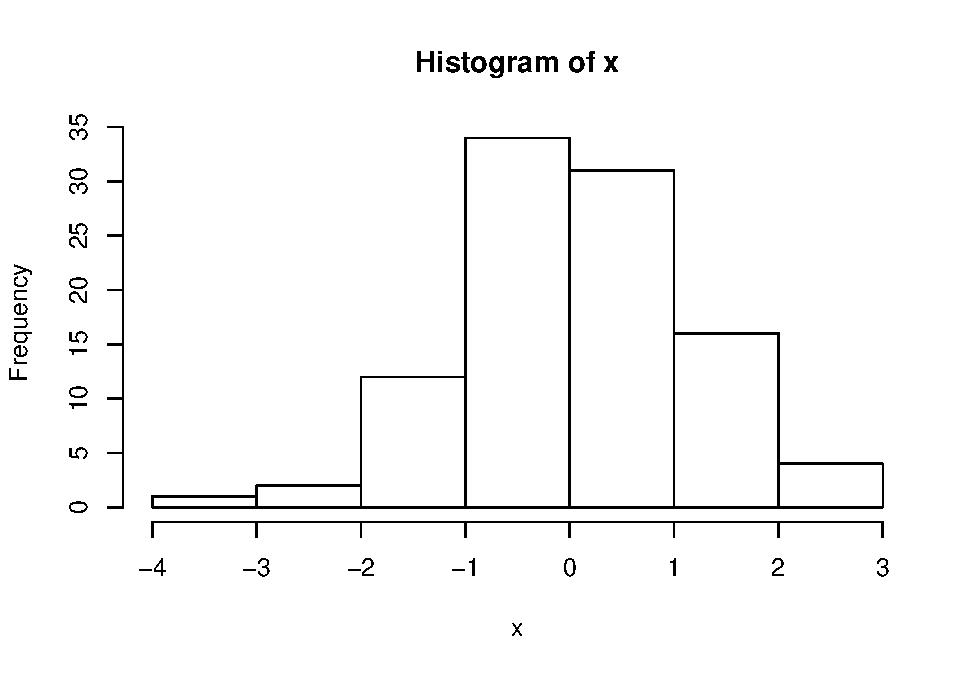
\includegraphics{HW1_files/figure-latex/hist-1.pdf}

\subsubsection{References}\label{references}


\end{document}
